\documentclass{article}

\usepackage{graphicx}
\usepackage{tikz}
\usepackage{tikzsymbols}
\usetikzlibrary{calc,patterns,shapes.geometric}
\pagestyle{empty}
\usepackage[margin=0pt]{geometry}
\geometry{papersize={14in,12in}}

\def\centerarc[#1](#2)(#3:#4:#5){\draw[#1] ($(#2)+({#5*cos(#3)},{#5*sin(#3)})$) arc (#3:#4:#5);}

\begin{document}
	\begin{figure}
		\centering
		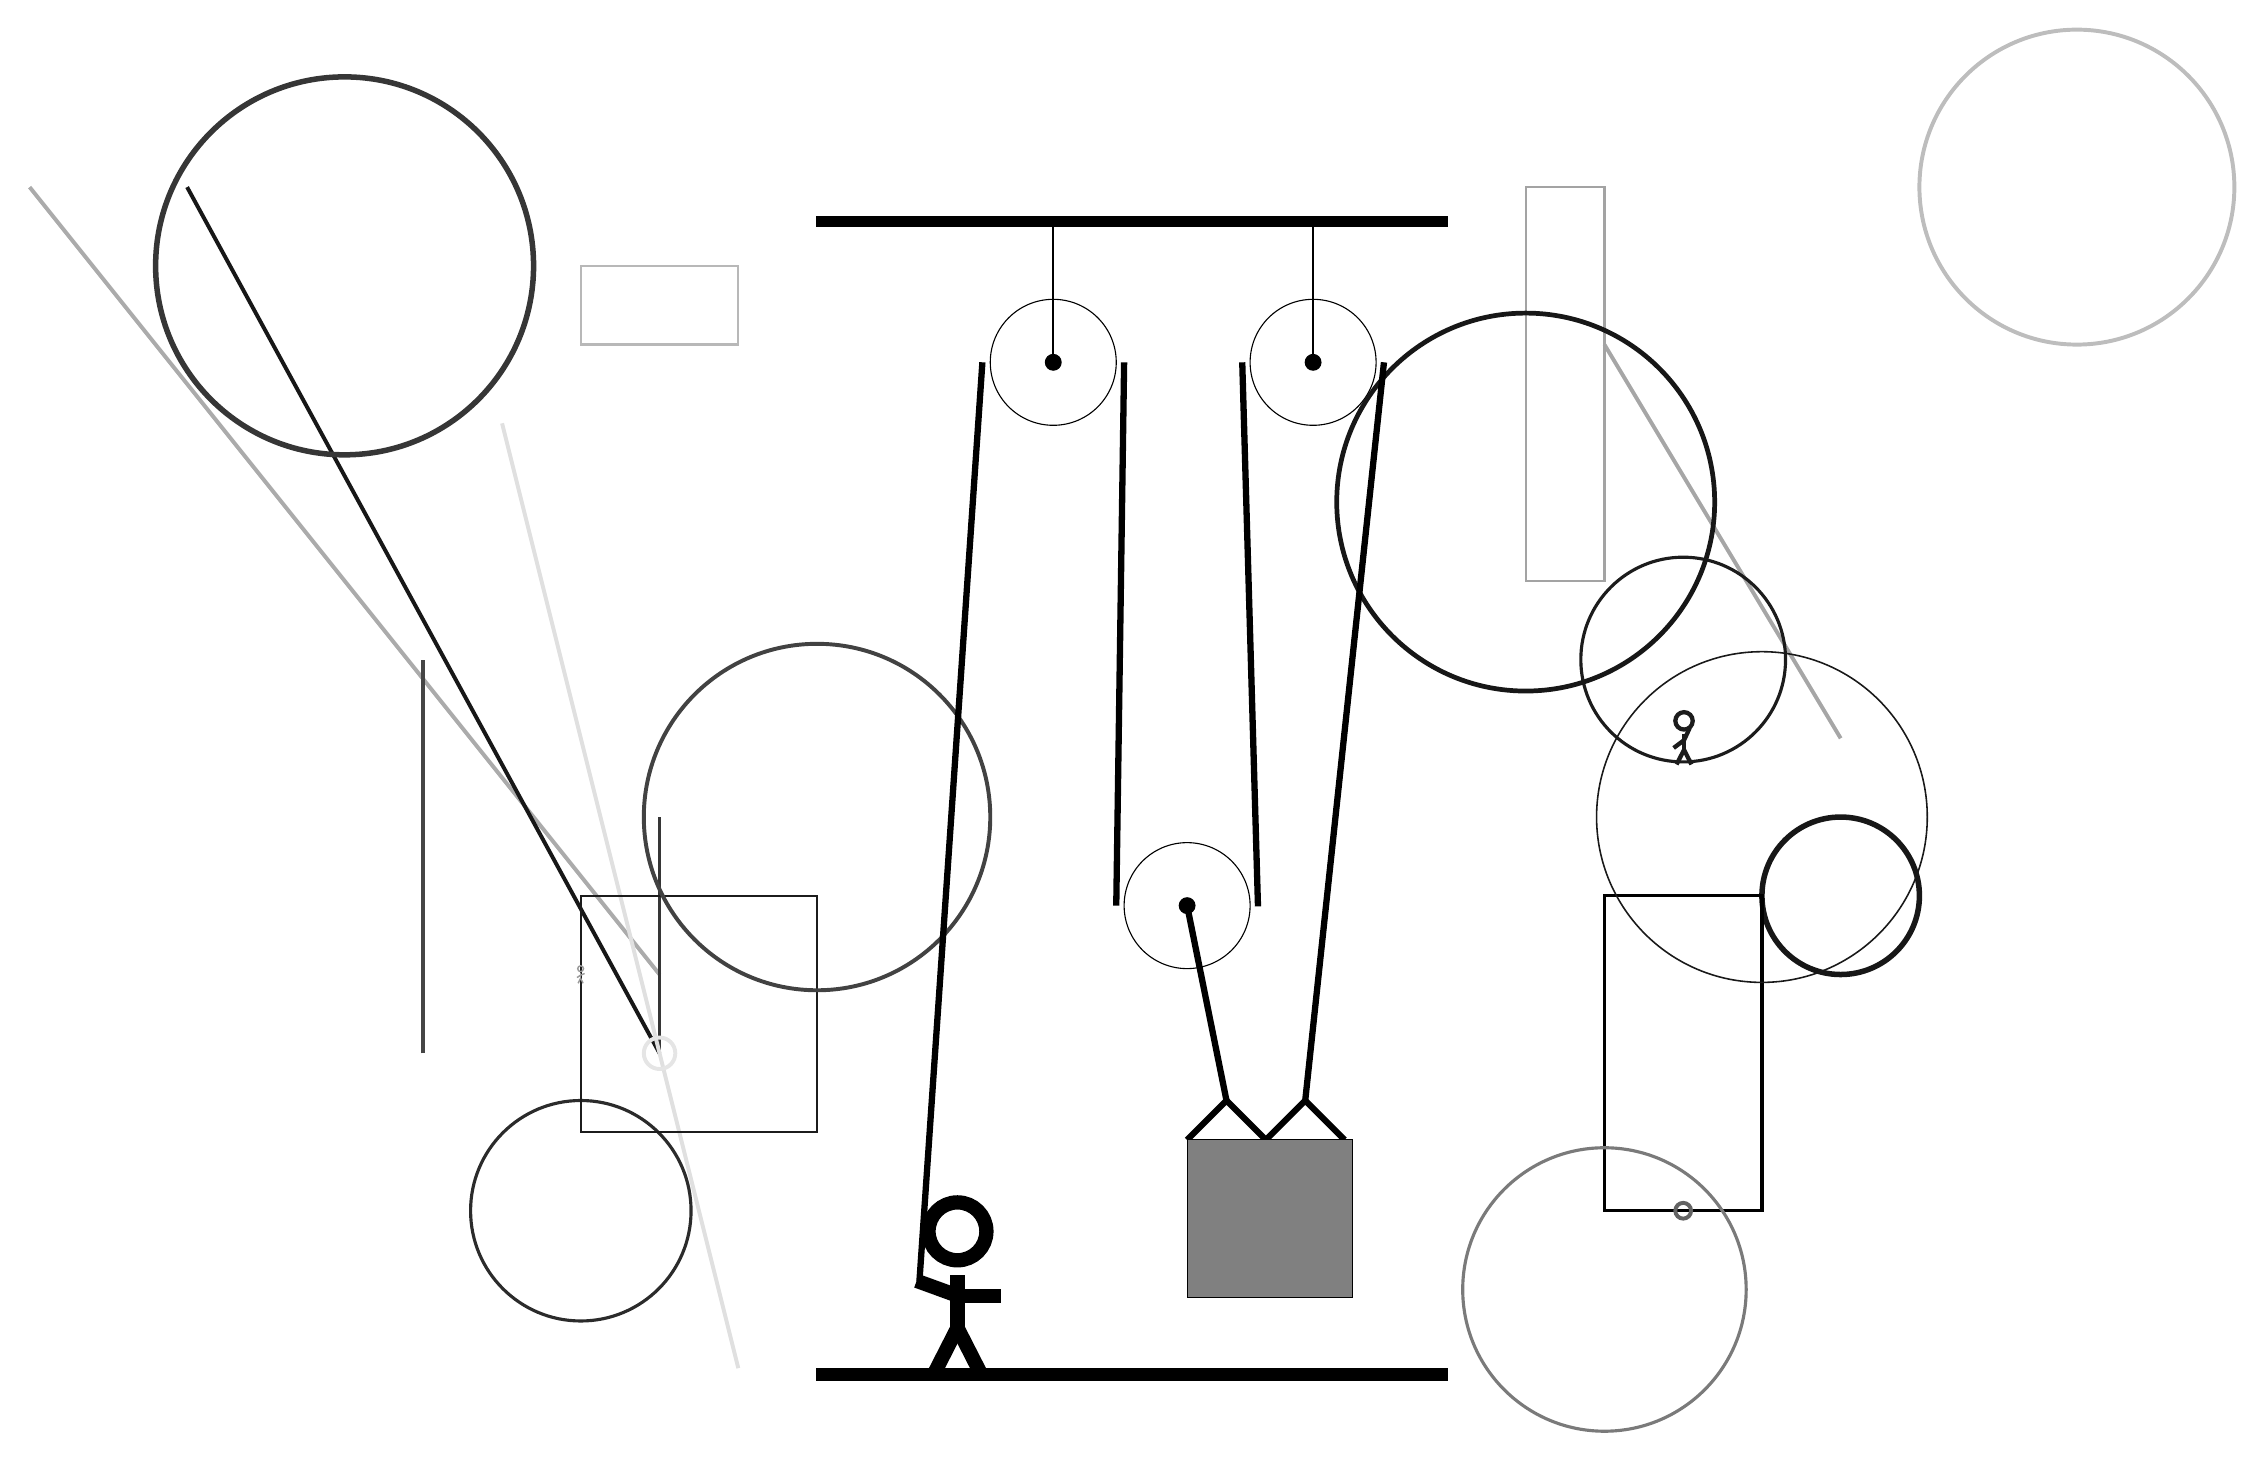
\begin{tikzpicture}
			%%%%% START %%%%%
			
			\draw[fill=black] (-2, 11.5) rectangle (6, 11.625);
			
			\draw (1, 9.775) circle (0.8);
			\draw[fill=black] (1, 9.775) circle (0.1);
			\draw[thick] (1, 9.775) -- (1, 11.5);
			
			\draw (4.3, 9.775) circle (0.8);
			\draw[fill=black] (4.3, 9.775) circle (0.1);
			\draw[thick] (4.3, 9.775) -- (4.3, 11.5);
			
			\draw (2.7, 2.875) circle (0.8);
			\draw[fill=black] (2.7, 2.875) circle (0.1);
			
			\draw[line width=0.8mm]  (2.7, -0.1) -- (3.2, 0.4) -- (3.7, -0.1) -- (4.2, 0.4) -- (4.7, -0.1);
			\draw[fill=black!50] (2.7, -0.1) rectangle (4.8, -2.1);
			
			\draw[line width=0.5mm, color=black!35](8, 10) -- (11, 5);
			
			\draw [line width=0.7mm, color=black!91](11, 3) circle (1.0);
			\node[line width=0.2mm, color=black!89] at (9, 5) {\Strichmaxerl[3][37][65]};
			\draw[line width=0.5mm, color=black!33](-4, 2) -- (-12, 12);
			\draw[line width=0.4mm, color=black!100] (8, 3) rectangle (10, -1);
			
			\draw [line width=0.4mm, color=black!52](8, -2) circle (1.8);
			\draw[line width=0.5mm, color=black!91](-4, 1) -- (-10, 12);
			\draw[line width=0.3mm, color=black!36] (8, 12) rectangle (7, 7);
			\draw [line width=0.4mm, color=black!83](-5, -1) circle (1.4);
			\draw [line width=0.5mm, color=black!61](9, -1) circle (0.1);
			\draw [line width=0.5mm, color=black!26](14, 12) circle (2.0);
			\draw[line width=0.4mm, color=black!79] (-4, 1) rectangle (-4, 4);
			\draw[line width=0.5mm, color=black!12](-3, -3) -- (-6, 9);
			\draw [line width=0.7mm, color=black!79](-8, 11) circle (2.4);
			\draw [line width=0.4mm, color=black!89](9, 6) circle (1.3);
			\draw[line width=0.2mm, color=black!89] (-2, 0) rectangle (-5, 3);
			\node[line width=0.6mm, color=black!40] at (-5, 2) {\Strichmaxerl[1][34][22]};
			\draw [line width=0.5mm, color=black!10](-4, 1) circle (0.2);
			\draw [line width=0.5mm, color=black!74](-2, 4) circle (2.2);
			
			\draw[line width=0.5mm, color=black!73](-7, 1) -- (-7, 6);
			\draw [line width=0.2mm, color=black!90](10, 4) circle (2.1);
			
			\draw[line width=0.3mm, color=black!28] (-3, 10) rectangle (-5, 11);
			
			\draw [line width=0.6mm, color=black!91](7, 8) circle (2.4);
			
			\draw[line width=0.8mm](-0.7, -1.9) -- (0.1, 9.775);
			\centerarc[line width=0.8mm](1, 9.775)(0:180:0.9);
			\draw[line width=0.8mm](1.9, 9.775) -- (1.8, 2.875);
			\centerarc[line width=0.8mm](2.7, 2.875)(180:370:0.9);
			\draw[line width=0.8mm] (3.6, 2.865) -- (3.4, 9.775);
			\centerarc[line width=0.8mm](4.3, 9.775)(0:180:0.9);
			\draw[line width=0.8mm](4.2, 0.4) -- (5.2, 9.775);
			\draw[line width=0.8mm] (3.2, 0.4) -- (2.7, 2.875);
			
			\node at (-0.2, -2) {\Strichmaxerl[10][-20][0]};
			
			\draw[fill=black] (-2, -3) rectangle (6, -3.15);
			
			%%%%% END %%%%%
		\end{tikzpicture}
	\end{figure}	
\end{document}